\chapter{Estado del arte}
\ihead[]{Capítulo 2: Estado del arte}
\label{ch:CH02-Estado-del-Arte}
%%%%%%%%%%%%%%%%%%%%%%%%%%%%%%%%%%%%%%%%%%
En este capítulo se presenta una revisión de \ac{SW} comerciales, empresas que se encargan de la venta de motores con sus respectivas especificaciones y trabajos de investigación relacionados con la caracterización de motores \ac{DC}. %asimismo se presentan tecnologías que serán tomados en cuenta para los conceptos de solución en capítulos posteriores
\section{Softwares comerciales}
    Se destacan 2 \ac{SW} que facilitan la estimación de parámetros de motores \ac{DC}, Con dichos \ac{SW} se piensa comparar los resultados que se obtengan con la solución que se planteará el capítulos posteriores.
    \subsection{Software ETAP}
        \ac{ETAP} es un \ac{SW} especializado en el análisis de sistemas eléctricos de potencia. Dentro de sus módulos, cuenta con un apartado dedicado a la estimación de parámetros de motores. Para ello, según lo indica la página oficial \autocite{etap}, utiliza técnicas de estimación matemática y ajuste de curvas para esta tarea, y requiere sólo datos de rendimiento del motor. También permite generar informes detallados y gráficos de los resultados, facilitando análisis de torque, corriente y eficiencia del motor \autocite{etap}. En la Figura \ref{fig:CH02_SW_ETAP} se presenta la interfaz del \ac{SW} referente a la caracterización de motores.
        \begin{figure}[!ht]
        \centering
        \begin{tabularx}{\linewidth}{>{\centering\arraybackslash}X}
            % Fila 1: imagen
            \begin{subfigure}[t]{0.5\linewidth}
                \centering
                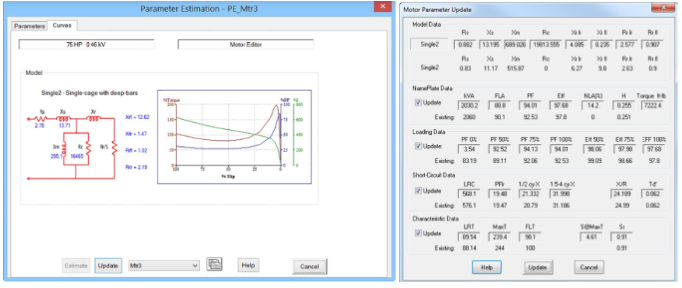
\includegraphics[width=\linewidth]{CHPTRS/CH02_SA/Fig/01_SWEtap.PNG}
            \end{subfigure}
        \end{tabularx}
        \caption{Imágenes extraídas de la página oficial de ETAP}
        \label{fig:CH02_SW_ETAP}
        \end{figure}
    
    \subsection{MATLAB/Motor Control Blockset}
        La herramienta \ac{MCB}, brindada por el \ac{SW} Matlab es utilizada para el diseño, simulación y prueba de sistemas de control de motores \ac{DC}. Entre sus principales funciones se destaca la simulación de motores con diferentes parámetros para analizar su comportamiento bajo diversas condiciones, el diseño de controladores de velocidad y torque utilizando técnicas de control de lazo cerrado y brinda documentación de proyectos y aplicaciones brindadas por la comunidad de temas relacionados con la estimación de motores \autocite{mathworks_motor_estimation}. \\
        \begin{figure}[!ht]
        \centering
        \begin{tabularx}{\linewidth}{>{\centering\arraybackslash}X}
            % Fila 1: imagen
            \begin{subfigure}[t]{0.5\linewidth}
                \centering
                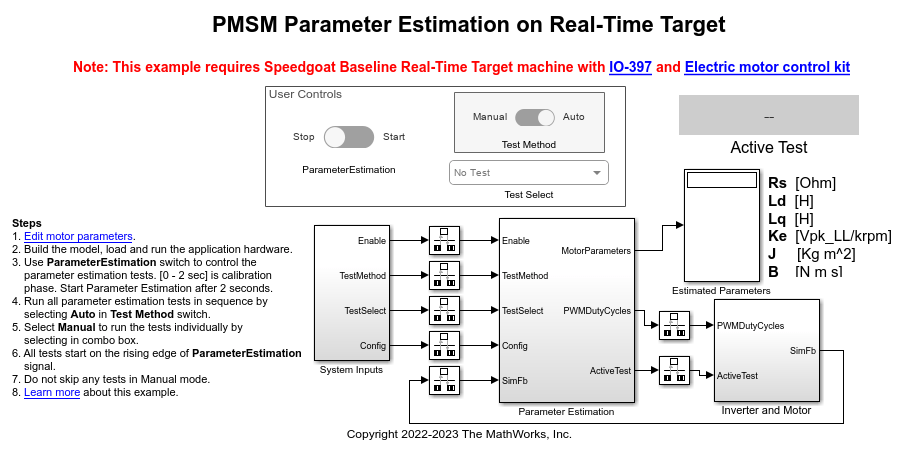
\includegraphics[width=\linewidth]{CHPTRS/CH02_SA/Fig/02_MatlabToolbox.png}
            \end{subfigure}
            \end{tabularx}
            \caption{Imagen extraída de la página de MathWorks \autocite{mathworks_motor_estimation}}
            \label{fig:CH02_SW_ETAP}
        \end{figure}
    A continuación se presenta en la Tabla \ref{tab:comparasion_sw} tabla comparativa entre los dos \ac{SW} presentados, se compararán el precio para adquirir estas herramientas, si cumplen con estimar los parámetros de motor y qué tanta documentación se le brinda al usuario. Toda información en dicha tabla ha sido consultada a las páginas oficiales de cada \ac{SW}.
    % Tabla adaptada con la plantilla "tabla_comparativa" (3 columnas)
    % NOTA: Ajusta {w1}+{w2}+{w3} <= 1 para evitar warnings.
    \begin{longtblr}[theme=pucp,
          label   = {tab:comparasion_sw},
          caption = {Comparación entre los dos \ac{SW} mencionados},
        ]{
          colspec   = {X[c,m]X[c,m]X[c,m]},
          column{1} = {wd=0.20\textwidth},
          column{2} = {wd=0.40\textwidth},
          column{3} = {wd=0.40\textwidth},
          rowhead = 1,
          rowfoot = 0,
          hlines,
          vlines,
        }
        Característica & \ac{ETAP} & MATLAB \textit{toolbox} \\
        Precio de la licencia
        & El \ac{SW} \ac{ETAP} tiene un precio modular, por lo que se deben comprar módulos separados para distintas características. \ac{ETAP} no publica precios directos; es necesario solicitar una cotización.
        & MATLAB opera con licencias cuyo precio varía según el tipo (individual, académico, etc.). La licencia anual base de MATLAB (con acceso a todas las herramientas) es de \$2{,}150, y el \ac{MCB} se vende por separado (puede llegar a \$1{,}500). El plan estudiantil más económico indicado por \textcite{mathworks_motor_estimation} cuesta \$55. \\
        Estimación de parámetros del motor
        & \ac{ETAP} se especializa en análisis de sistemas eléctricos de potencia e incluye un apartado para estimar parámetros de motores \ac{DC} como resistencia, inductancia y par.
        & MATLAB/\ac{MCB} ofrece herramientas completas para estimación de parámetros de motores, con entornos de simulación e interfaces de hardware para diseño de control y pruebas en tiempo real. \\
        Soporte y documentación
        & \ac{ETAP} ofrece soporte extenso: ayuda en vivo, capacitaciones, seminarios web y foro dedicado.
        & MATLAB/\ac{MCB} cuenta con documentación completa, foros de usuarios, soporte técnico de MathWorks y abundantes tutoriales en línea. \\
    \end{longtblr}

\section{Empresas de confianza}
    En esta sección, se analizarán dos empresas internacionales que ofrecen a sus clientes los parámetros técnicos de sus motores en hojas de especificaciones antes de la compra de sus productos.
    \subsection{Maxon}
        Maxon ofrece soluciones de sistemas de accionamiento mecatrónico y uno de sus componentes de mayor interés son los motores \ac{DC}. Estos componentes se destacan por su alta precisión, fiabilidad y adaptabilidad a diversas aplicaciones industriales, médicas, aeroespaciales y de movilidad. Los motores \ac{DC} de Maxon se usan en entornos donde la identificación de parámetros precisos, como torque, velocidad y eficiencia, es crítica para un rendimiento óptimo, especialmente en tareas de automatización y robótica \autocite{maxon_group}. Adicionalmente, buscando en la página oficial, al cotizar un motor de esta marca puedes realizar distintas combinaciones de componentes como \textit{drivers}, encoders pero lo principal es que por cada motor, te brindan una lista de especificaciones, de las cuales se destacan las que ayudarán al control del motor. En la Figura \ref{fig:CH03_MOTOR_MAXON} se muestra la cotización de uno de los modelos de motor \ac{DC} y en la Tabla \ref{tab:motor_maxon} se brindan las especificaciones de dicho motor.
    
    \begin{figure}[H]
        \centering
        \begin{tabularx}{\linewidth}{>{\centering\arraybackslash}X}
            % Fila 1: imagen
            \begin{subfigure}[t]{0.5\linewidth}
                \centering
                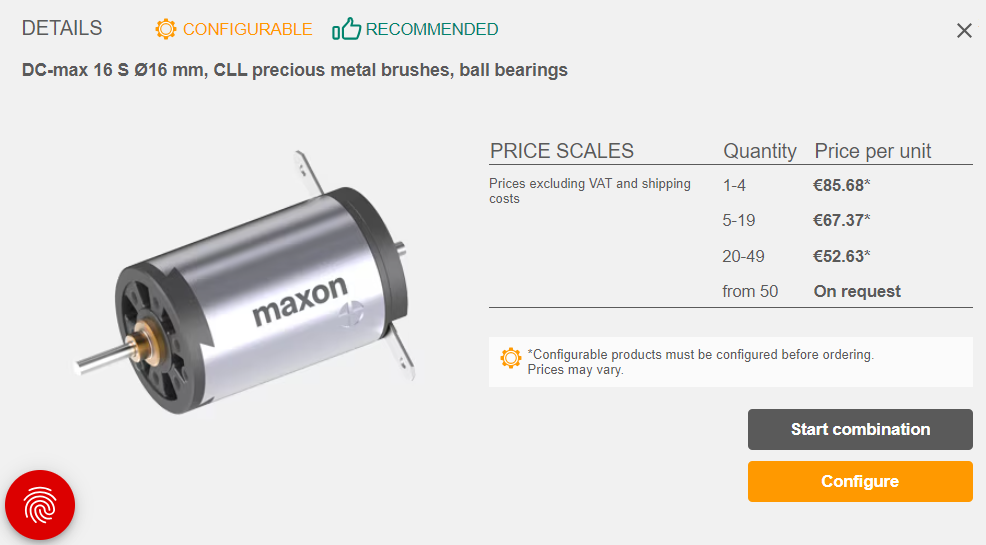
\includegraphics[width=\linewidth]{CHPTRS/CH02_SA/Fig/03_MaxonMotor.PNG}
            \end{subfigure}
        \end{tabularx}
        \caption{Imagen referencial del motor cotizado en la página de MAXON}
        \label{fig:CH03_MOTOR_MAXON}
    \end{figure}
    \begin{table}[H]
        \centering
        \caption{Parámetros brindados por la empresa MAXON al momento de elegir un motor\\(modelo DC-max 16)}
        \begin{tblr}{
              cell{1}{3} = {c},
              cell{2}{3} = {c},
              cell{3}{3} = {c},
              cell{4}{3} = {c},
              cell{5}{3} = {c},
        }
        \hline
        Características              & Valor            &  \\
        \hline
        Resistencia terminal         & \SI{4.1}{\ohm}   &  \\
        Inductancia terminal         & \SI{0.14}{\mH}   &  \\
        Constante de par             & 7,19 mNm/A       &  \\
        Constante de velocidad       & 1330 rpm/V       &  \\
        Gradiente de velocidad/par   & 758 rpm/mNm      &  \\
        Constante de tiempo mecánico & 8,87 ms          &  \\
        Inercia del rotor            & 1,12 $gcm^2$     &
        \end{tblr}
        \caption*{\small\textit{Nota: Información adaptada de un motor cotizado en la página de \href{https://www.maxongroup.com/es-es}{Maxon}, revisada el día 25 de setiembre del 2024 \autocite{maxon_group}}}
        \label{tab:motor_maxon}
    \end{table}

\subsection{Zhaowei}
    ZHAOWEI es una empresa que se especializa en el diseño, desarrollo y fabricación de motores \ac{DC} con escobillas, así como en sistemas de transmisión y soluciones personalizadas para la industria. Se enfoca principalmente en la venta de motores de alta precisión y componentes relacionados afines para el accionamiento y medición de parámetros de estos \autocite{zhaowei_dc_motor} Lo destacable de la empresa es que, al igual que fabricantes como \textcite{zhaowei_dc_motor}, proporcionan los parámetros técnicos detallados de sus motores antes de la compra, lo cual es importante para que los clientes puedan evaluar si el motor cumple con sus requisitos específicos. Algo a detallar es que al momento de ingresar a cotizar un motor, dichos parámetros se encuentran ligados a una tolerancia de casi el 20 \% para la mayoría de estos y en algunos casos no muestran los valores de algunos parámetros. En la Figura \ref{fig:CH03_MOTOR_ZHAOWE} se muestran los principales parámetros de uno de los modelos de motor \ac{DC} de la página principal de esta empresa y en la Tabla \ref{tab:motor_zhaowei} se muestran los valores de los parámetros del motor cotizado.

    \begin{figure}[H]
        \centering
        \begin{tabularx}{\linewidth}{>{\centering\arraybackslash}X}
            % Fila 1: imagen
            \begin{subfigure}[t]{0.8\linewidth}
                \centering
                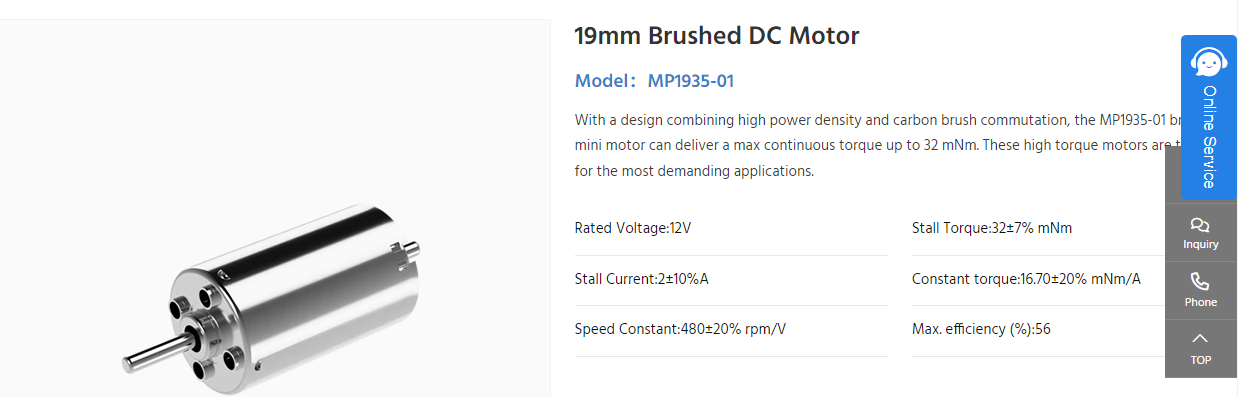
\includegraphics[width=\linewidth]{CHPTRS/CH02_SA/Fig/04_ZhaoweiMotor.PNG}
            \end{subfigure}
        \end{tabularx}
        \caption{Imagen referencial del motor cotizado en la página de Zhaowei}
        \label{fig:CH03_MOTOR_ZHAOWE}
    \end{figure}
    \begin{table}[H]
        \centering
        \caption{Parámetros brindados por la empresa ZHAOWEI del motor cotizado en su página web}
        \begin{tblr}{
          cell{1}{3} = {c},
          cell{2}{3} = {c},
          cell{3}{3} = {c},
          cell{4}{3} = {c},
          cell{5}{3} = {c},
        }
        \hline
        Características                    & Valor            &  \\
        \hline
        Resistencia terminal de fase       & \SI{4.5}{\ohm}   &  \\
        Inductancia terminal de fase       & \text{N.A.}      &  \\
        Constante de par                   & 13,1 mNm/A       &  \\
        Constante de velocidad             & 684 rpm/V        &  \\
        Gradiente de velocidad/par         & 243,5 rpm/mNm    &  \\
        Constante de tiempo mecánico       & -- ms            &  \\
        Inercia del rotor                  & 4 $gcm^2$        &
        \end{tblr}
        \caption*{\small\textit{Nota: Información adaptada de un motor cotizado en la página de \href{https://es.zwgearbox.com/}{Zhaowei}, revisada el día 25 de setiembre del 2024 \autocite{zhaowei_dc_motor}}}
        \label{tab:motor_zhaowei}
    \end{table}


Para la validación de los resultados del estimador diseñado, se utilizará un motor proveniente de alguna de las dos empresas mencionadas, dado que estas empresas proporcionan una hoja técnica con los valores de los parámetros del motor. Además, se planea aplicar métodos empíricos y utilizar algún \ac{SW} para comparar cuál de estas tres metodologías ofrece resultados más cercanos a la respuesta real y determinar cuál de ellas es la mejor opción para hallar los parámetros.
 
\section{Artículos académicos:}
    A continuación se presentan 3 artículos enfocados en caracterizar motores de corriente continua, cada uno de ellos muestra distintas técnicas para lograr estimar los modelos de motores \ac{DC}, pero lo que se comparte en cada una de estas publicaciones es la efectividad de sus modelos al compararlos con los datos obtenidos por un motor real. 
    \subsection{Identificación de parámetros de motores de \ac{DC} usando respuesta en frecuencia}
        En este artículo\textcite{vollmecke_parameter_identification} propone la estimación de parámetros de motores \ac{DC} utilizando la respuesta en frecuencia para reconstruir la función de transferencia del motor mediante la aproximación de los polos que caracterizan la dinámica del sistema. En la Figura \ref{fig:CH03_Diagrama_Bode} se presenta el diagrama de Bode del sistema una vez determinados los polos. Posteriormente, estos se emplean para calcular los parámetros del motor utilizando las constantes de tiempo de respuesta del sistema: en el dominio eléctrico, para determinar los valores de la resistencia e inductancia; y en el dominio mecánico, para calcular la inercia y el factor de viscosidad del eje del motor.
        \begin{figure}[h!]
            \centering
            \begin{tabularx}{\linewidth}{>{\centering\arraybackslash}X}
                % Fila 1: imagen
                \begin{subfigure}[t]{0.8\linewidth}
                    \centering
                    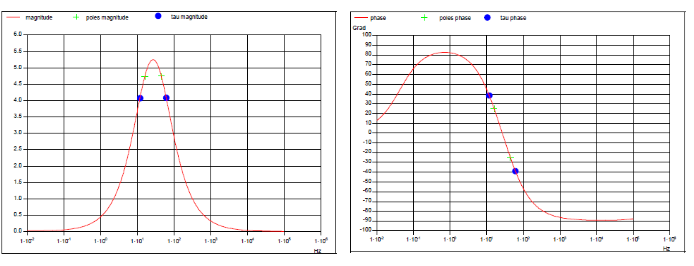
\includegraphics[width=\linewidth]{CHPTRS/CH02_SA/Fig/05_RespFrecuencia.PNG}
                \end{subfigure}
            \end{tabularx}
            \caption{Diagrama de Bode que muestra la identificación de los polos del motor}
            \label{fig:CH03_Diagrama_Bode}
        \end{figure}

    \subsection{Identificador algebraico de parámetros mecánicos de un motor \ac{DC}}
        En un artículo publicado por Academia Journals, se presenta un método económico para identificar únicamente los parámetros mecánicos de motores \ac{DC}, específicamente la inercia del eje y el coeficiente de viscosidad. Según \textcite{parametros_mecanicos}, se implementa el modelo del motor \ac{DC} junto con un identificador algebraico de parámetros en MATLAB/SIMULINK, como se ilustra en la Figura \ref{fig:CH03_ESTIMADOR_MECANICO}, donde se simula el comportamiento del sistema en condiciones ideales. Para la implementación experimental, se utiliza el circuito mostrado en la misma figura, en el cual un microcontrolador Arduino UNO procesa las mediciones de velocidad y corriente para determinar los parámetros del motor \ac{DC}, enviándolos posteriormente a MATLAB/SIMULINK. Un sensor infrarrojo con \textit{encoder} mide la velocidad del motor, mientras que un circuito simple con una resistencia permite medir la corriente.
        \begin{figure}[H]
            \centering
            \begin{tabularx}{\linewidth}{>{\centering\arraybackslash}X}
                % Fila 1: imagen
                \begin{subfigure}[t]{0.6\linewidth}
                    \centering
                    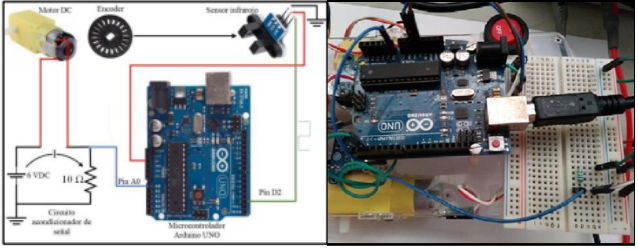
\includegraphics[width=\linewidth]{CHPTRS/CH02_SA/Fig/06_Antecedente1.PNG}
                \end{subfigure}
            \end{tabularx}
            \caption{Implementación experimental para la toma de datos}
            \label{fig:CH03_ESTIMADOR_MECANICO}
        \end{figure}

        A continuación se presentan los resultados de la estimación que obtuvo \textcite{parametros_mecanicos}, donde se destaca que al ser una implementación con componentes bastante económicos y sin la ayuda de filtros, sólo se logra estimar correctamente el coeficiente de viscosidad, más no el momento de inercia del eje del motor debido a que no se filtró correctamente el ruido en la toma de datos. Esto como se logra ver en la comparación de parámetros entre el real y el que fue estimado. El efecto de la inercia nunca llega a converger con el resultado obtenido por el estimador. Esto se presenta en la Figura \ref{fig:CH03_RESULTADOS_MECANICOS}.
        \begin{figure}[H]
            \centering
            \begin{tabularx}{\linewidth}{>{\centering\arraybackslash}X}
                % Fila 1: imagen
                \begin{subfigure}[t]{0.6\linewidth}
                    \centering
                    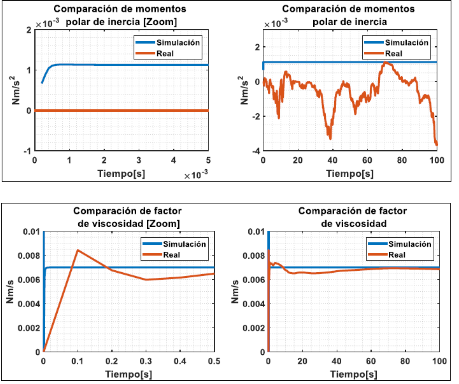
\includegraphics[width=\linewidth]{CHPTRS/CH02_SA/Fig/07_Antecedentes2.PNG}
                \end{subfigure}
            \end{tabularx}
            \caption{Resultados de la estimación de parámetros mecánicos}
            \label{fig:CH03_RESULTADOS_MECANICOS}
        \end{figure}

    \subsection{Sistema de identificación paramétrica para motores \ac{DC} usando método de mínimos cuadrados}
        El siguiente artículo proviene de una publicación de 2 institutos mexicanos y trata de un sistema diseñado para identificar los parámetros que describen la función de transferencia de un motor de corriente continua. El sistema consta de una tarjeta para la adecuación de señales, una tarjeta de adquisición de datos y una aplicación de computadora que implementa el algoritmo de mínimos cuadrados usando un programa creado en MATLAB. Las señales que requirieron medir incluyen la velocidad angular en radianes por segundo, la corriente de armadura en amperios y el voltaje de alimentación en voltios. Se muestra la relación matemática entre la función de transferencia del motor de corriente continua y las funciones de transferencia de velocidad y corriente. En la Figura \ref{fig:CH03_DIAGRAMA_ESQ_MEX} presenta el diagrama de conexiones que usaron \textcite{est_matlab_art_mexicano} para la adquisición de datos de motores \ac{DC}. Además, en la Figura \ref{fig:CH03_INTERFAZ_MEX} se muestra la interfaz que desarrolló su equipo para realizar la estimación de parámetros del motor.
    \begin{figure}[!ht]
        \begin{tabularx}{\linewidth}{*{2}{>{\centering\arraybackslash}X}}
            % FILA-1, COL-1 (imagen izquierda)
            \begin{subfigure}[t]{0.45\textwidth}
                \centering
                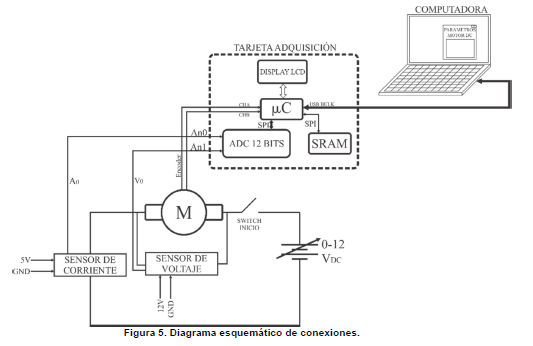
\includegraphics[width=.9\linewidth,height=4cm,keepaspectratio]{CHPTRS/CH02_SA/Fig/08a_DiagramaConexiones.PNG}
            \end{subfigure}
            &
            % FILA-1, COL-2 (imagen derecha)
            \begin{subfigure}[t]{0.45\textwidth}
                \centering
                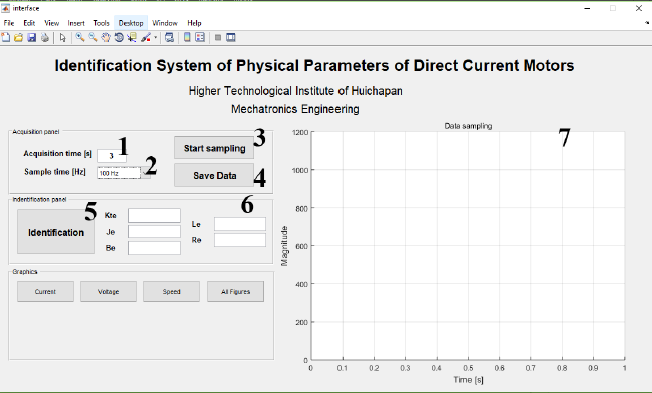
\includegraphics[width=.9\linewidth,height=4cm,keepaspectratio]{CHPTRS/CH02_SA/Fig/08b_Interfaz.PNG}
            \end{subfigure}
            \\
            % FILA-2 (captions individuales)
            \begin{subfigure}[t]{0.8\linewidth}
                \caption{Diagrama esquemático de conexiones para toma de datos de motores \ac{DC}}
                \label{fig:CH03_DIAGRAMA_ESQ_MEX}
            \end{subfigure}
            &
            \begin{subfigure}[t]{0.8\linewidth}
                \caption{Interfaz propuesta para el procesamiento y ejecución del algoritmo de estimación}
                \label{fig:CH03_INTERFAZ_MEX}
            \end{subfigure}
        \end{tabularx}
        \caption{Diseño propuesto por \textcite{est_matlab_art_mexicano} para la estimación de parámetros de motores \ac{DC}}
        \label{fig:figura_con_subfiguras}
    \end{figure}

